\documentclass[10pt, conference, compsocconf]{IEEEtran}

% packages
\usepackage{algorithm}
\usepackage{algorithmic}
\usepackage{amsfonts} % for R symbol (the set of real numbers)
\usepackage{color}
\usepackage[pdftex]{graphicx}
\usepackage[bookmarks=false]{hyperref}
\hypersetup{colorlinks=true,linkcolor=black,citecolor=black,filecolor=black,urlcolor=blue}
\usepackage{mathtools}
\usepackage{multirow}
\usepackage{stmaryrd} % for llbracket and rrbracket
\usepackage{subcaption}
\DeclarePairedDelimiter{\ceil}{\lceil}{\rceil}
\DeclarePairedDelimiter{\floor}{\lfloor}{\rfloor}

% new commands
\newcommand{\todo}[1]{\marginpar{\parbox{18mm}{\flushleft\tiny\color{red}\textbf{TODO}:
      #1}}}

\newcommand{\note}[1]{
  \color{blue}\emph{[Note: #1]}
  \color{black}
}

\begin{document}

\title{Predicting computational reproducibility of scientific pipelines using collaborative filtering}

\author{Soudabeh Barghi, Lalet Scaria, Tristan Glatard\\
  Department of Computer Science and Software Engineering\\ Concordia University, Montreal, Quebec, Canada\\
  {first.last}@concordia.ca\\
  $^*$ These authors have contributed equally
}

\maketitle

\begin{abstract}
\end{abstract}


\section{Introduction}

Computational reproducibility, the property through which
computational results can be recomputed over time and
space~\cite{stodden}, has become a critical component of scientific
methodology with the rise of the reproducibility crisis in several
domains~\cite{xxx}. Among the factors hampering computational
reproducibility, infrastructural characteristics such as the operating
system play an important role. In neurosciences, our primary field of
interest, several studies have shown the effect of the operating
system on computational results. However, conducting such
reproducibility studies at scale is cumbersome due to the execution
time of data analysis pipelines, which easily exceeds a few hours.

In this paper we investigate approximate methods to predict the
reproducibility of a computational analysis from the first files that
it produces. Our main intuition is that reproducibility errors are
caused by a reduced number of factors that originate in the analysis
pipeline and input data. 

% Computational reproducibility is an issue, for instance among
% different operating systems (refer to Glatard FINF 2015,
% Gronenschild 2012).

% Scientific data analysis pipeline executions are long (give examples
% from neuroimaging).

% Refer to Germain et al 2008.

% Define subjects, pipelines.

% Problem: predict the reproducibility of pipeline files from other
% subjects and the first files produced by a pipeline. Restrict the
% study to binary classification.




\section{Method}

% What is specific to our problem compared to regular collaborative filtering:
%+ subjects are equivalent to users. Not all subjects have the same input data. Anatomical variability, acquisition variability (e.g., 1 subject may have multiple T1s).
%+ files are produced in a specific order (movies aren't),
% which add constraints on the training set (cannot sample late files and not early ones).
%+ utility matrix is not sparse: we can potentially populate it completely. Which means that we can decide precisely which samples we need (active sampling). Therefore we can take the first row and first column to avoid cold start issues.

\subsection{Collaborative filtering using ALS}

% Summarize Koren, Bell and Volinsky: https://dl.acm.org/citation.cfm?id=1608614

% Explain that you have binary classes (rounding)

% Biases

\subsection{Sampling the Training Set}

% Explain all sampling techniques (maybe rename 4, 5, and 6)
% 1. random unreal (baseline)
% 2. columns
% 3. rows
% 4. random real
% 5. random diagonal
% 6. random triangular
% For every method, show a training matrix to illustrate for a given ratio. 

\section{Dataset}

We acquired data about the computational reproducibility of analysis
pipelines of the Human Connectome Project~\cite{general-hcp}. We
processed a set S of 94 subjects randomly selected in the S500 HCP
release~\todo{URL} in three execution conditions with different
versions of the CentOS operating system (5.?, 6.? and 7.?), using the
PreFreesurfer, Freesurfer, PostFreesurfer and fMRIVolume pipelines
described in~\cite{hcp-pipelines} and available at \todo{URL}. For
each pipeline, we identified the set F of files produced for all
subjects in all conditions. For each condition pair and each pipeline,
we computed a binary difference matrix D of size $|F|\times|S|$, where $D_{i,j}$ is true
if file $i$ of subject $j$ was different in each condition. Rows of
$M$ are ordered by ascending file modification time in the pipeline.

Figure~\ref{fig:pre-freesurfer-5-7} shows the difference matrix
obtained for the PreFreesurfer pipeline\todo{Remove title from figure,
  remove color scale, add axes labels.}. The computational
reproducibility of the PreFreesurfer pipeline varies across subjects,
which motivates our study. Nevertheless, some files behave
consistently across all subjects, leading to complete black or white
lines. The ratio of positive elements in this matrix is
\todo{x}\%. Similar matrices were obtained with this pipeline for
CentOS~6 vs CentOS~7 and for CentOS~5 vs CentOS~6, see
Figures~\ref{fig:pre-freesurfer-5-6} and~\ref{fig:pre-freesurfer-5-7}.

\begin{figure}
  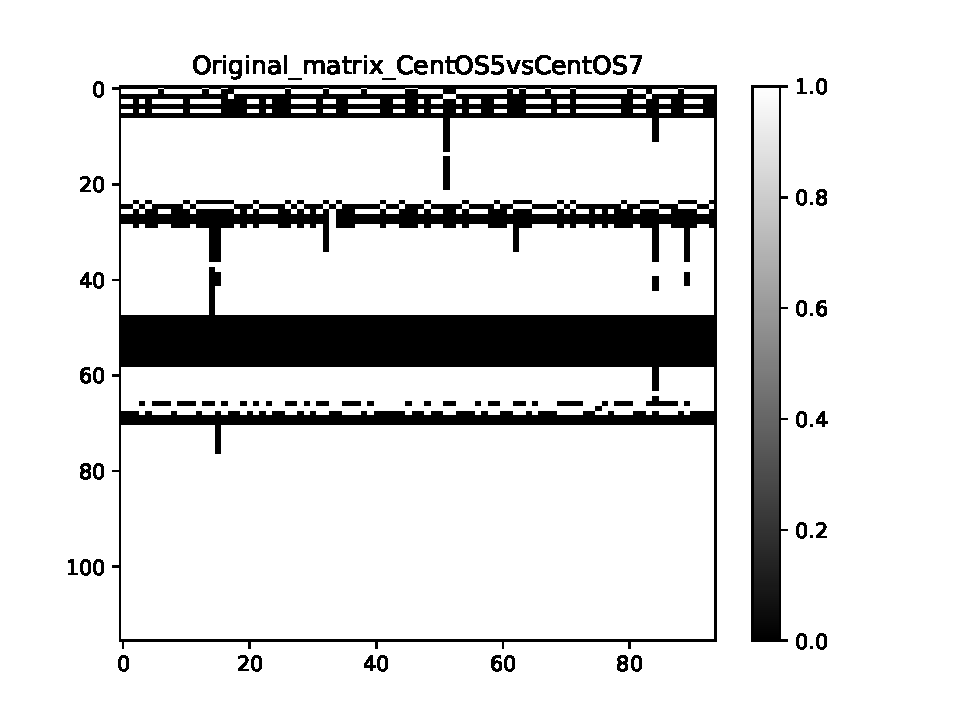
\includegraphics[width=\columnwidth]{figures/original_matrix_CentOS5vsCentOS7.pdf}
  \caption{Difference matrix, PreFreesurfer pipeline, CentOS~5 vs CentOS~7.}
  \label{fig:pre-freesurfer-5-7}
\end{figure}

% Describe your dataset: pipeline(s) used, input data, operating systems (CentOS5, 6, 7), matrix.

% 1. Prefreesurfer (what you have)
% 2. Freesurfer, with the same subjects as in Prefreesurfer.
% 3. PostFreesurfer
% 4. fmriVolume

\section{Results}

% Present your results: accuracy, ROC curves, transparency matrix, factors. 

% Try with different numbers of factors. 

\section{Discussion}

% Not all subjects behave the same, which motivates the Big Data approach. 

% Which sampling method is best

% Interpreting the factors? Factors reflect the pipeline definition. 

% How can this be used in practice

% What are the limitations

\section{Conclusion}

% Summary of the results and discussion. The take-home message.

\section*{Acknowledgment}

\bibliographystyle{IEEEtran}
\bibliography{IEEEabrv,biblio.bib}


\end{document}
